\section{Supporting Mathematics}\label{app.model.math}
%===================================================================================================
\subsection{Exponential Duration Assumption in Compartmental Models}\label{app.model.math.exp}
Let $\lambda$ be the fixed exit rate from compartment $A$, which is assumed to be homogeneous.
Then $\delta \sim \lambda e^{-\lambda \delta}$ is % TODO: (*) double check this
the exponentially distributed duration time in the group.
\paragraph{Mean \& Median Duration}
The mean duration is $\mu = 1/\lambda$ and the median is $m = \log(2)/\lambda \approx 0.69\,\mu$.
Thus, if 50\% of individuals progress from compartment $A$ to $B$ by time $\tau$ (median duration),
the exit rate $\lambda$ is given by $\log(2)/\tau$.
\paragraph{Collapsing Compartments in Series}
Let compartments $A$ and $B$ be in series, with exit rates $\lambda_A$ and $\lambda_B$ respectively.
Collapsing $A$ and $B$ into $AB$ will sum the mean durations: $\delta_{AB} = 1/\lambda_A + 1/\lambda_B$;
thus, the exit rate from $AB$ will be $\lambda_{AB} = 1/(1/\lambda_A + 1/\lambda_B)$.
\paragraph{Collapsing Compartments in Parallel}
Let compartments $A$ and $B$ be in parallel, with exit rates $\lambda_A$ and $\lambda_B$ respectively.
Collapsing $A$ and $B$ into $AB$ will sum the exit rates: $\lambda_{AB} = \lambda_A + \lambda_B$;
thus, the mean duration in $AB$ will be $\delta_{AB} = 1/(\lambda_A + \lambda_B)$.
%===================================================================================================
\subsection{Beta Approximation of the Binomial (BAB) Distribution}\label{app.model.math.bab}
Numerous model parameters and calibration targets represent population proportions.
Such proportions can be estimated as $\rho = n / N$, where
$N$ is the sample size and $n$ is the number of individuals with the characteristic of interest.
The uncertainty around $n$ is then given by the binomial distribution:
\begin{equation}\label{eq:binom}
  p(n) = {N \choose n} \, \rho^{n}{(1 - \rho)}^{N - n}
\end{equation}
However, \eqref{eq:binom} is only defined for discrete values of $n$.
It is more convenient to have a continuous distribution for $\rho$,
for sampling parameters and evaluating the likelihood of calibration targets,
since compartmental models can have non-whole-number population sizes.
For this purpose, I use a beta approximation of the binomial distribution (BAB):
\begin{equation}\label{eq:beta}
  p(\rho) =
    \frac{\Gamma(\alpha+\beta)}{\Gamma(\alpha)\,\Gamma(\beta)}\,
    \rho^{\alpha-1}{(1 - \rho)}^{\beta-1}
\end{equation}
with $\alpha = N\,\rho$ and $\beta = N\,(1-\rho)$.
Unlike the approximation by a normal distribution,
the beta distribution ensures that $\rho \in [0,1]$.
Figure~\ref{fig:bab} illustrates the approximation for
$N = \{10,20,40\}$ and $\rho = \{0.01,0.1,0.5\}$.
\begin{figure}
  \centering
  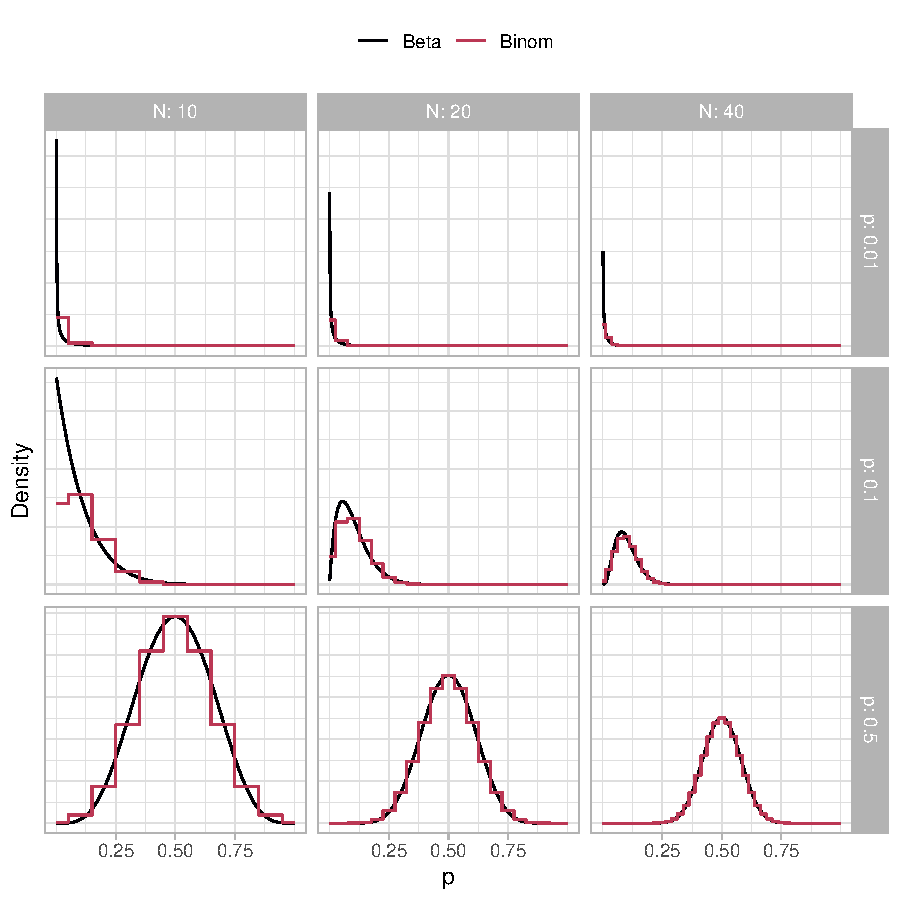
\includegraphics[width=.8\linewidth]{bab}
  \caption{Beta approximation of the binomial distribution (BAB)}
  \label{fig:bab}
\end{figure}
%===================================================================================================
\subsection{Joint Sampling with Relational Constraints}\label{app.model.math.jsam}
Figure~\ref{fig:jsam.bias} illustrates the posterior (sampled) distributions
for variables $X_1$, $X_2$, $X_3$, having uniform priors but subject to $X_1 < X_2 < X_3$.
Three approachs to enforcing $X_1 < X_2 < X_3$ were explored:
\begin{itemize}
  \item \textbf{joint:}
    sample $X_1$, $X_2$, $X_3$ simultaneously;
    then discard any samples failing $X_1 < X_2 < X_3$.
  \item \textbf{forward:}
    sample $X_1$;
    then sample $X_2$ until $X_1 < X_2$;
    then sample $X_3$ until $X_2 < X_3$.
  \item \textbf{backward:}
    sample $X_3$;
    then sample $X_2$ until $X_2 < X_3$;
    then sample $X_1$ until $X_1 < X_2$.
\end{itemize}
All three methods result in a different posterior \vs the prior,
but the forward and backward methods
severely distort the distributions for $X_3$ and $X_1$, respectively,
while leaving the distributions for $X_1$ and $X_3$ unchanged.
By contrast, the joint method influences the posterior distributions of each variable
in a more ``equitable'' way, which is preferred.
\begin{figure}[h]
  \centering
  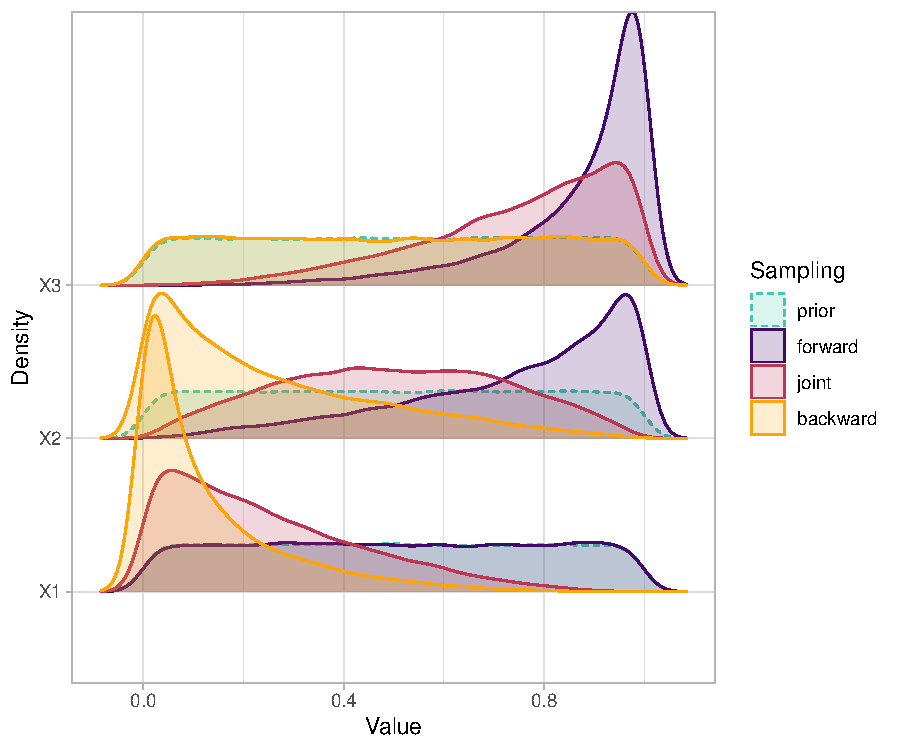
\includegraphics[width=.6\linewidth]{jsam.bias}
  \caption{Illustration of different sampling biases when enforcing $X_1 < X_2 < X_3$}
  \label{fig:jsam.bias}
\end{figure}
%===================================================================================================
\subsection{Fitting Distributions}\label{app.model.math.fit}
Uncertainty distributions for all parameters and calibration targets were estimated by
fitting a parametric distribution to specified quantiles.
Let $f\,(x\mid\theta)$ be
the probability density function of random variable~$x$ (parameter or target)
given distribution parameters $\theta$.
Then $F\,(x\mid\theta) = \int_0^x f(\tau)\,d\tau$ is the cumulative distribution function,
and $Q(p\mid\theta) = F^{\,-1}(p\mid\theta)$ is the quantile function.
Our objective is to estimate $\theta$, given a set of quantiles
(\eg $q = \{q_{2.5},q_{97.5}\}$ for the 95\%~CI).
For each estimation, I minimized%
\footnote{Using \hreftt{docs.scipy.org/doc/scipy/reference/optimize.minimize-lbfgsb.html}}
the following error function:
\begin{equation}
  J\,(\theta) = \sum_i {\big|\,q_i - Q(p_i\mid\theta)\,\big|}^{\,\omega}
\end{equation}
where $\omega$ can specify absolute differences ($\omega=1$) or squared differences ($\omega=2$)
to improve convergence.
Distribution fit was validated visually using a plot of
the distribution quantiles $Q(p_i\mid\theta)$ \vs the target quantiles $q_i$,
overlaid on the density distribution $f\,(x\mid\theta)$; \eg Figure~\ref{fig:distr.fit}.
\begin{figure}[h]
  \centering
  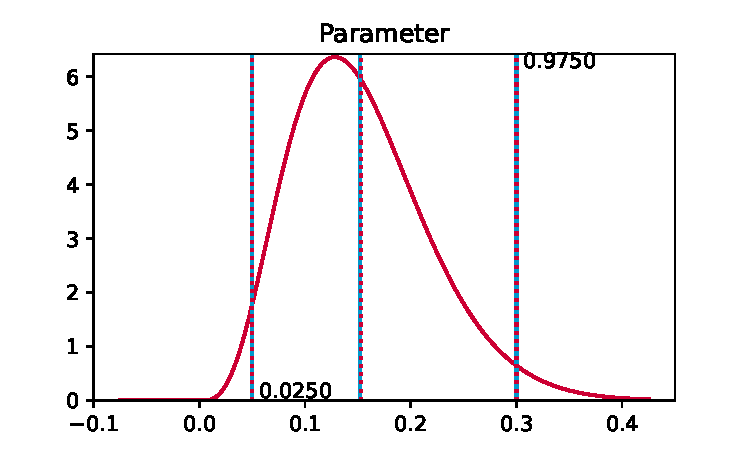
\includegraphics[width=.6\linewidth]{distr.fit}
  \caption{Example distribution fitting validation plot}
  \label{fig:distr.fit}
  \floatfoot{BAB distribution fit to $\{q_{2.5} = .05, q_{97.5} = .30\}$;
    blue solid lines: target quantiles $q_i$;
    red dotted lines: distribution quantiles $Q(p_i\mid\theta)$;
    red solid line: density distribution $f\,(x\mid\theta)$.}
\end{figure}
